% -*- latex -*-
%%%%%%%%%%%%%%%%%%%%%%%%%%%%%%%%%%%%%%%%%%%%%%%%%%%%%%%%%%%%%%%%
%%%%%%%%%%%%%%%%%%%%%%%%%%%%%%%%%%%%%%%%%%%%%%%%%%%%%%%%%%%%%%%%
%%%%
%%%% This text file is part of the source of 
%%%% `Parallel Computing'
%%%% by Victor Eijkhout, copyright 2012/3/4/5
%%%%
%%%% mpi-functional.tex : about functional parallelism
%%%%
%%%%%%%%%%%%%%%%%%%%%%%%%%%%%%%%%%%%%%%%%%%%%%%%%%%%%%%%%%%%%%%%
%%%%%%%%%%%%%%%%%%%%%%%%%%%%%%%%%%%%%%%%%%%%%%%%%%%%%%%%%%%%%%%%

%\input chapters/mpi-idiom-func
\Level 0 {The SPMD model}

MPI programs conform\footnote{Usually, but not necessarily.}
to the \acf{SPMD} model, where each processor runs the same executable.
This running executable we call a \indexterm{process}.

When MPI was first written, 20 years ago, it was clear what a processor
was: it was what was in a computer on someone's desk, or in a rack.
If this computer was part of a networked cluster, you called it a \indexterm{node}.
So if you ran an MPI program, each node would have one MPI process;
%
\begin{figure}[ht]
  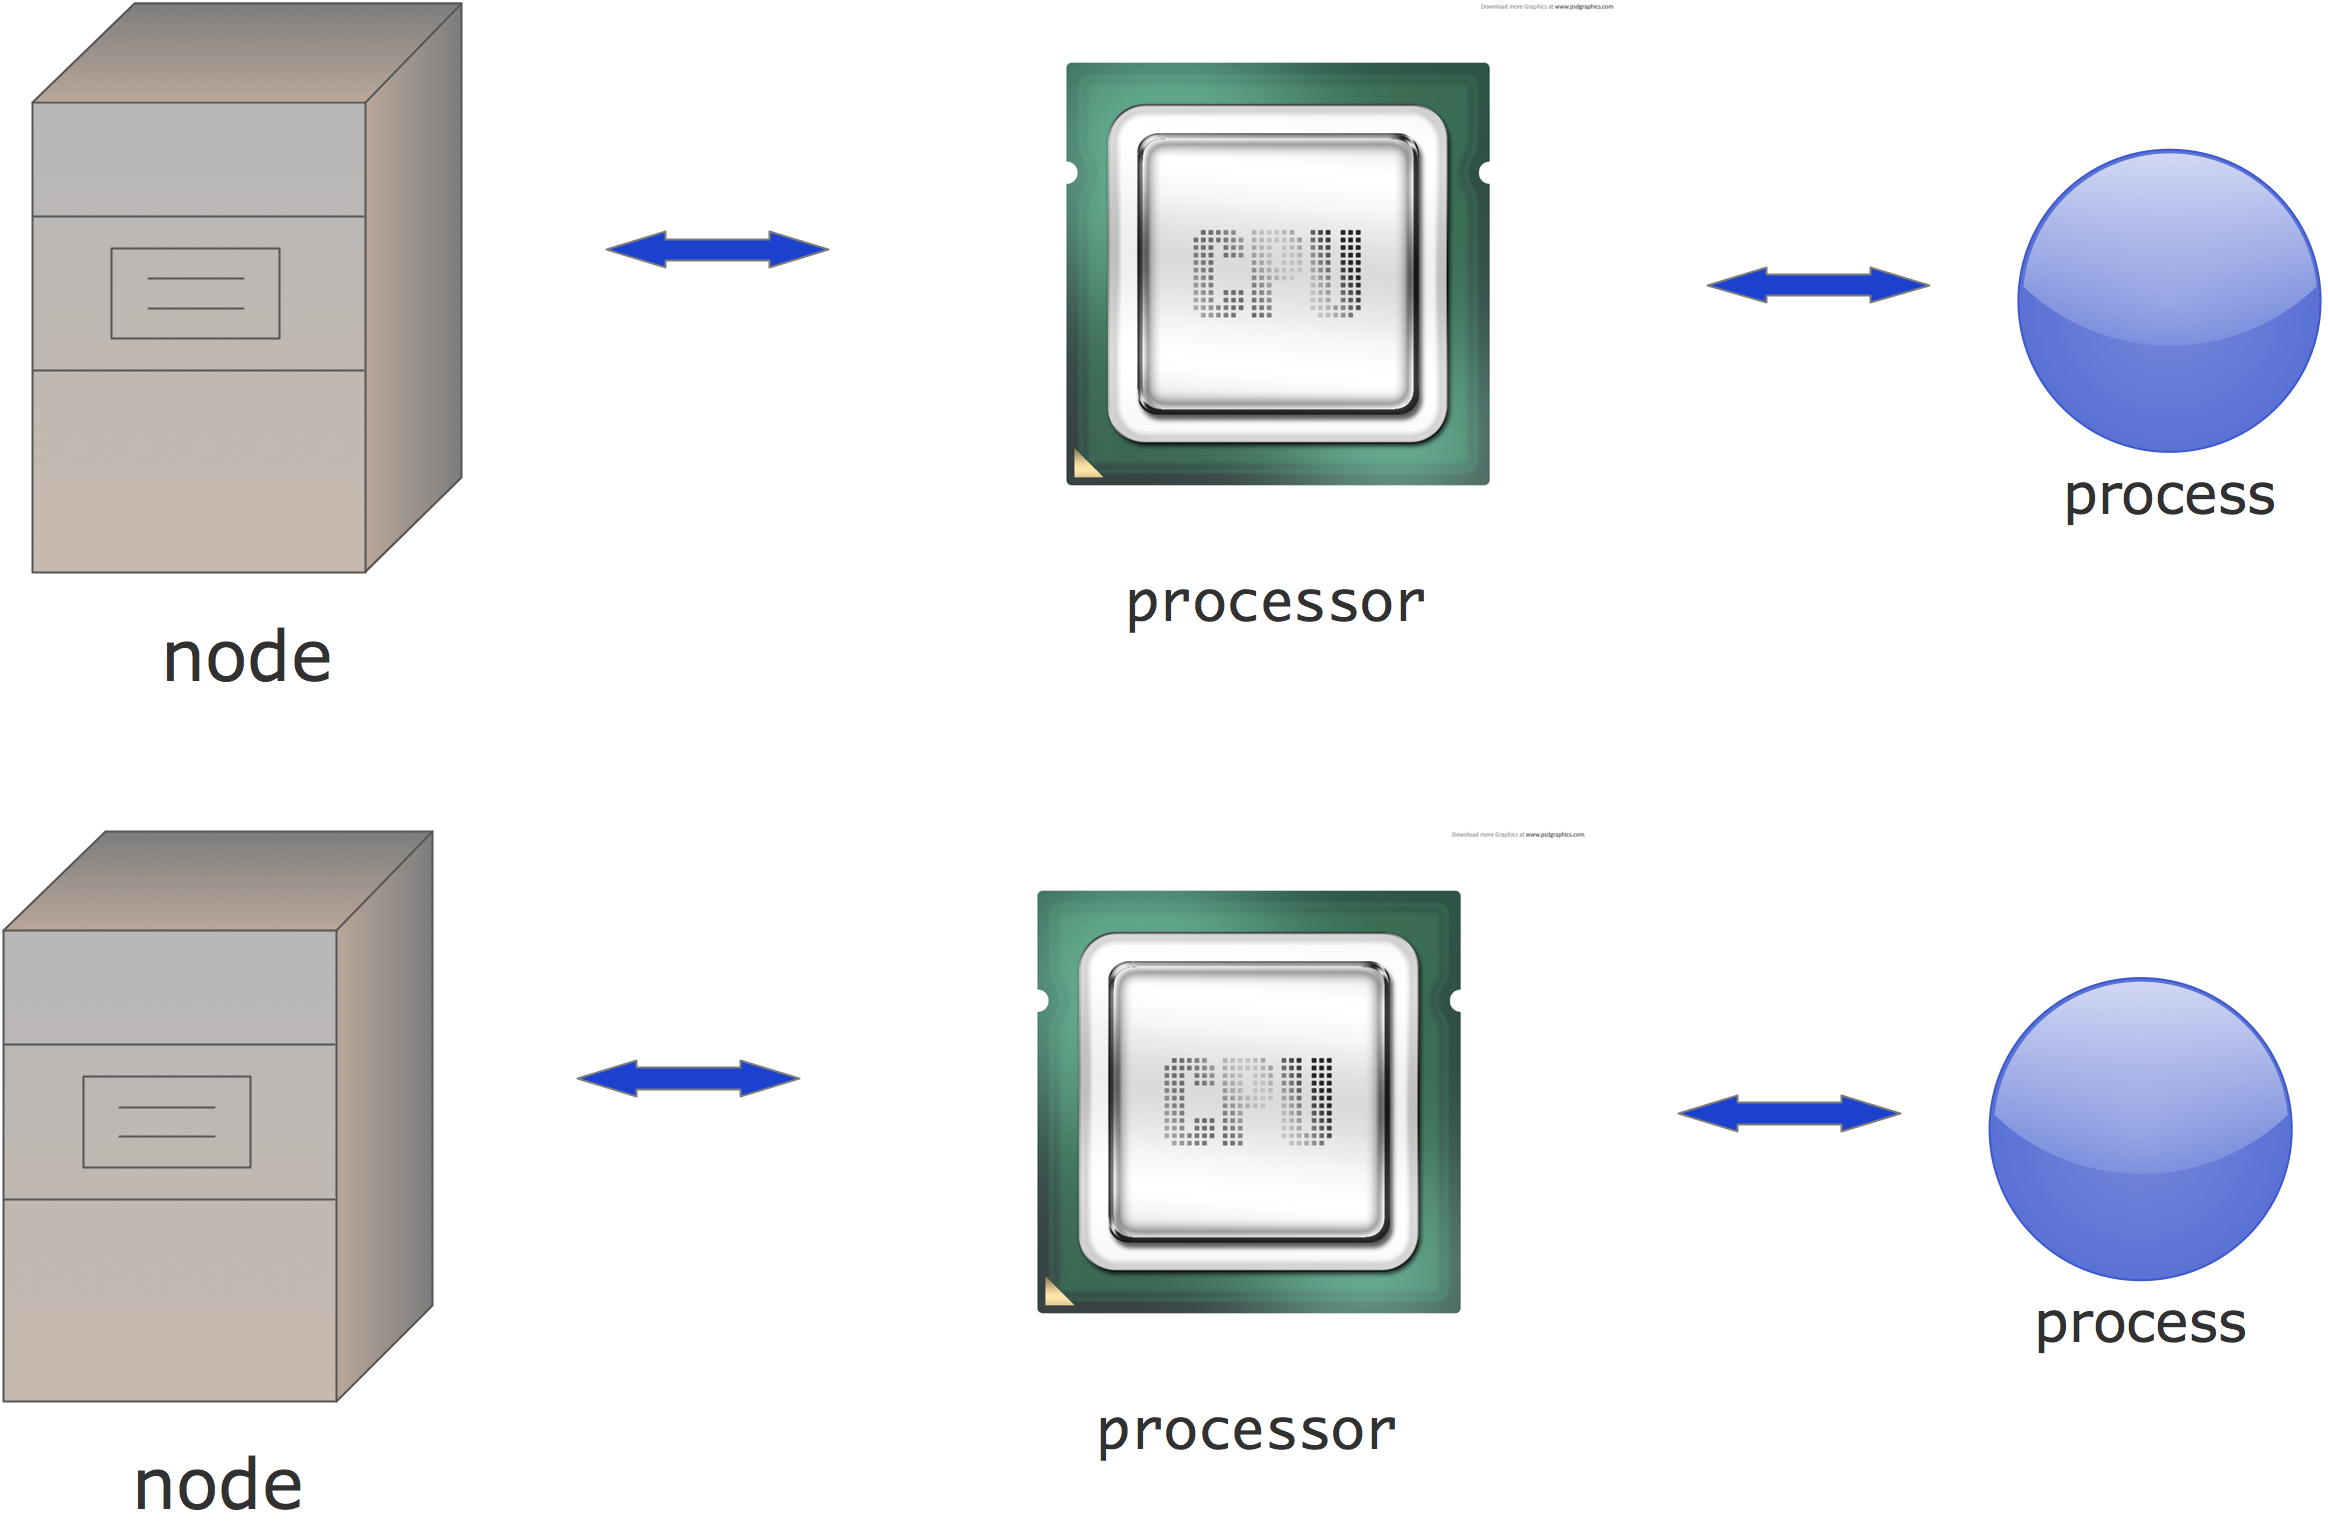
\includegraphics[scale=.11]{mpi-node1}
  \caption{Cluster structure as of the mid 1990s}
  \label{fig:oldmpi}
\end{figure}
%
figure~\ref{fig:oldmpi}.

These days the situation is more complicated.
You can still talk about a node in a cluster, but now a node can contain
more than one processor chip (sometimes called a \indexterm{socket}),
and each processor chip probably has multiple
\emph{cores}\index{core}.
%
\begin{figure}[ht]
  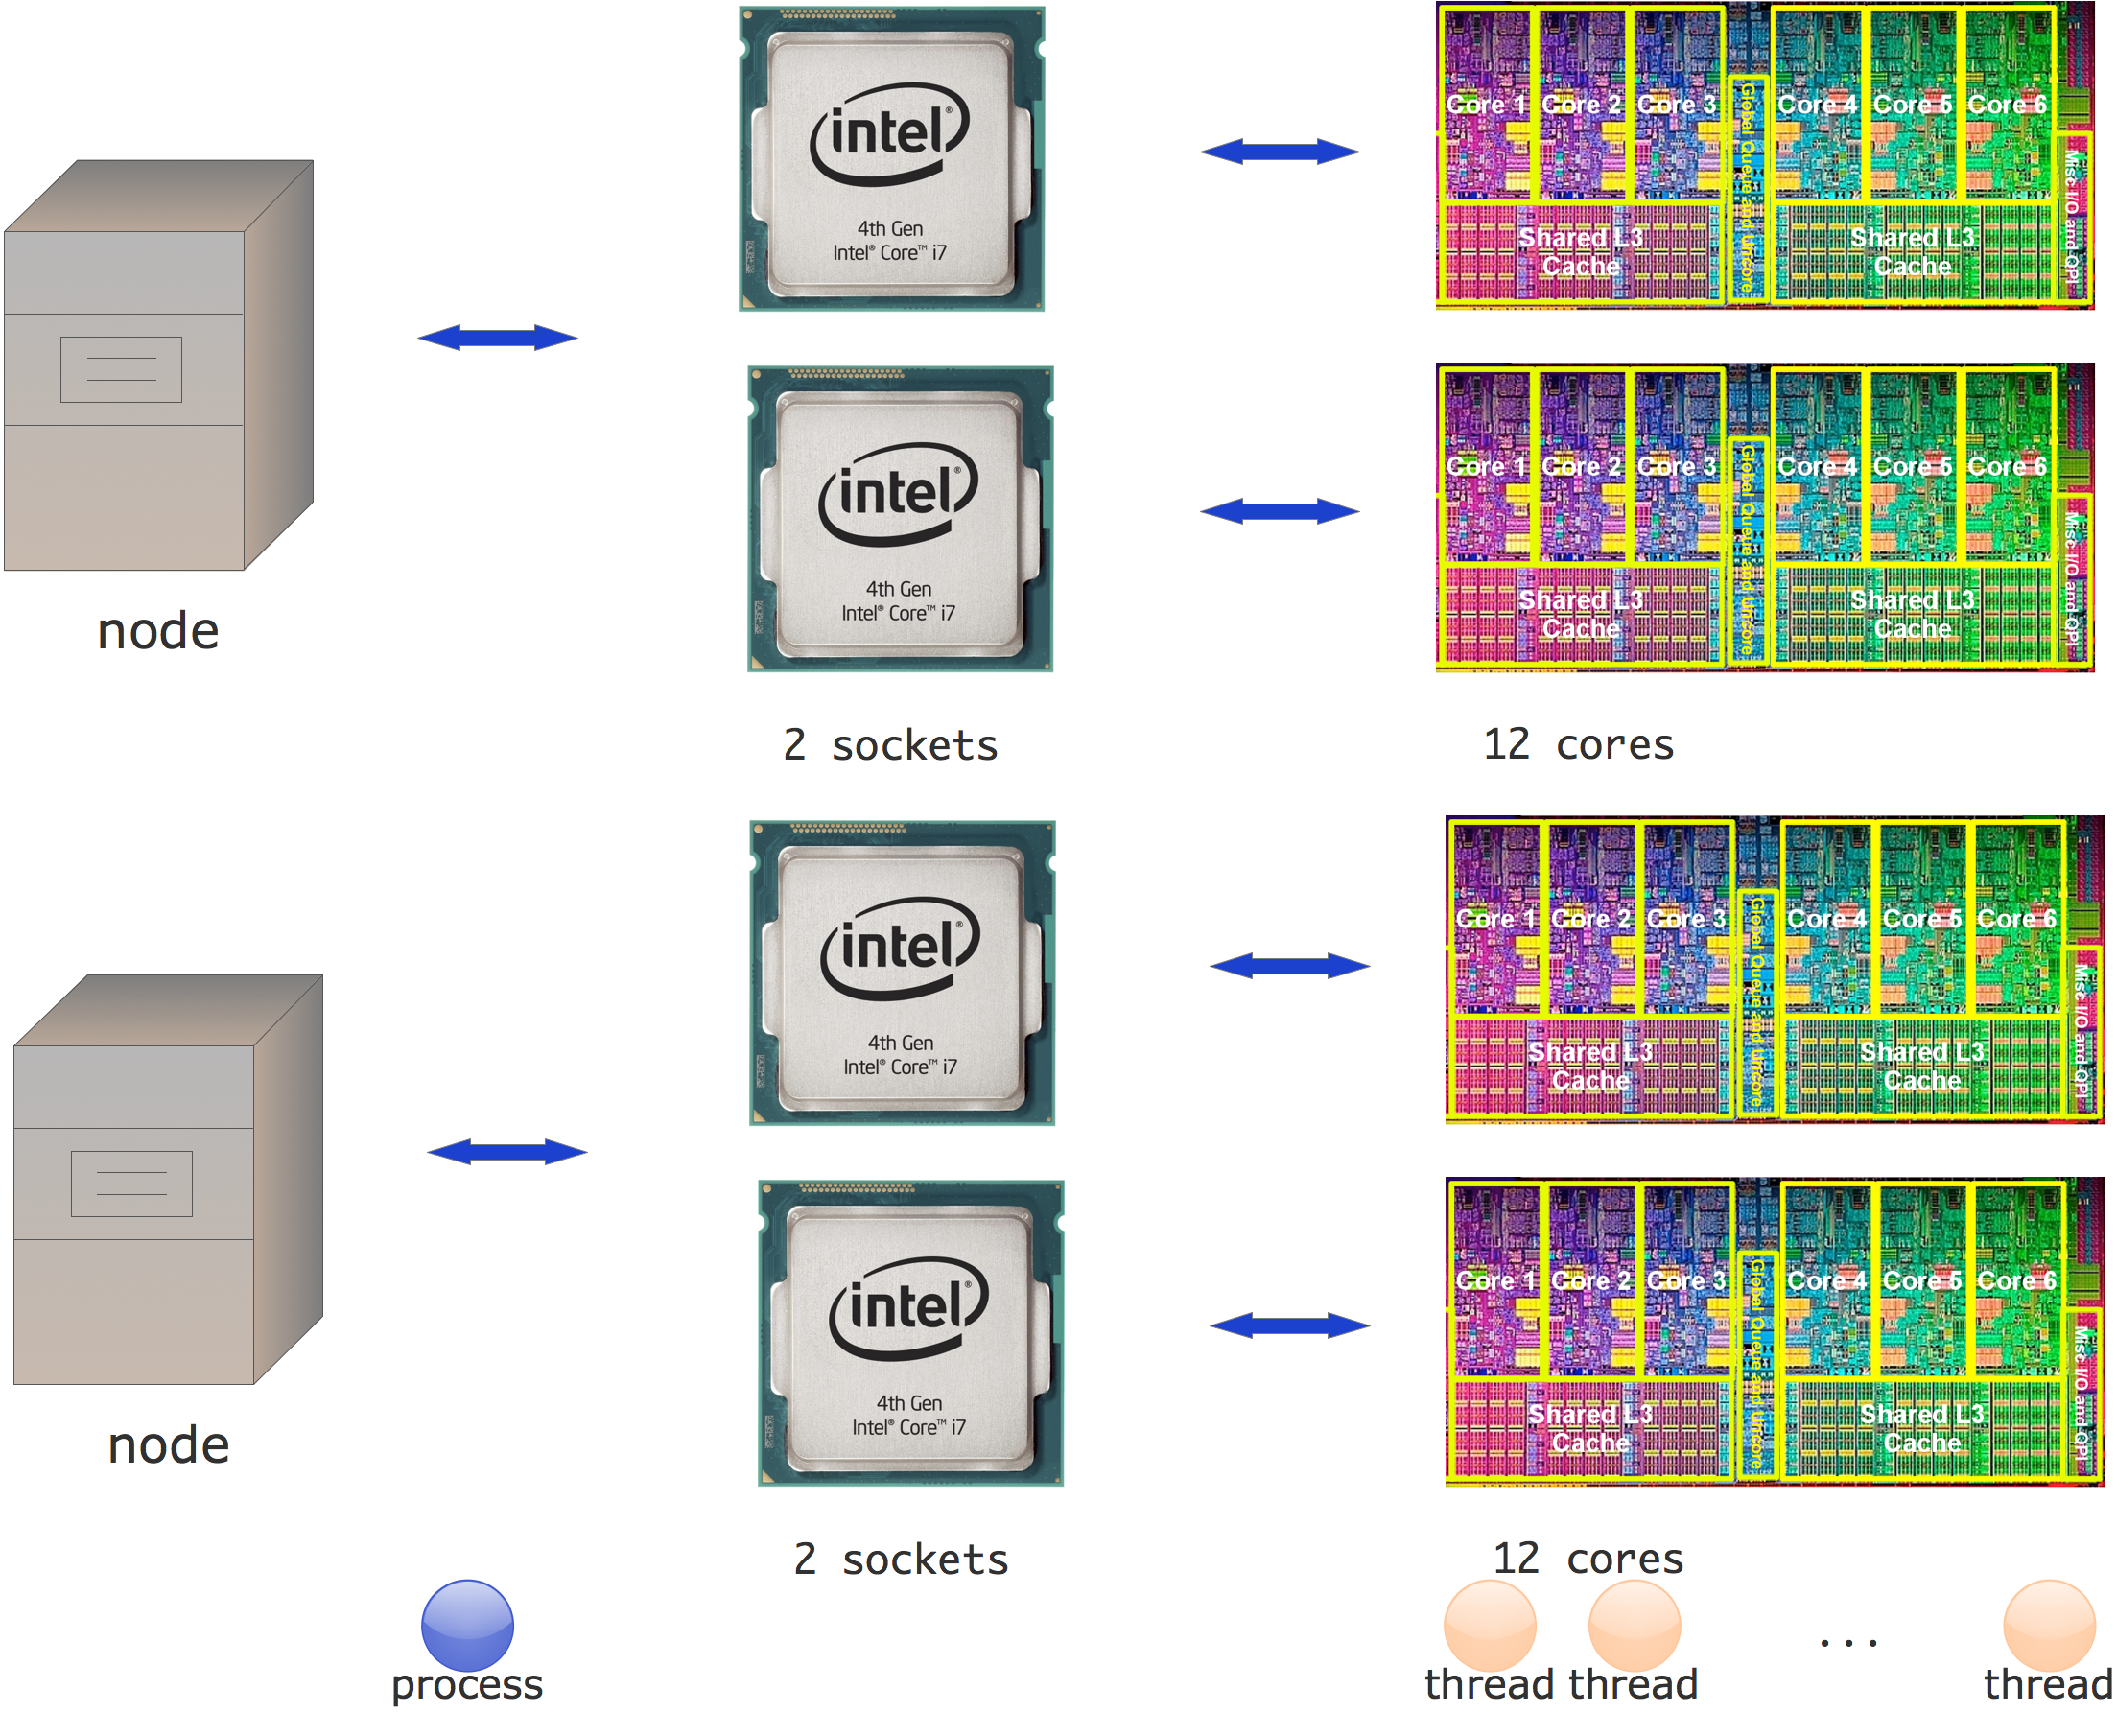
\includegraphics[scale=.11]{mpi-node3}
  \caption{Hybrid cluster structure}
  \label{fig:hybridmpi}
\end{figure}
%
Figure~\ref{fig:hybridmpi} shows how you could explore this using a mix
of MPI between the nodes, and a shared memory programming system on the nodes.

However, since each core can act like an independent processor,
you can also have multiple MPI processes per node. To MPI the cores look
like the old completely separate processors. This is the `pure MPI'
model of figure~\ref{fig:purempi} which we will use in most of this part
of the book.
%
\begin{figure}[ht]
  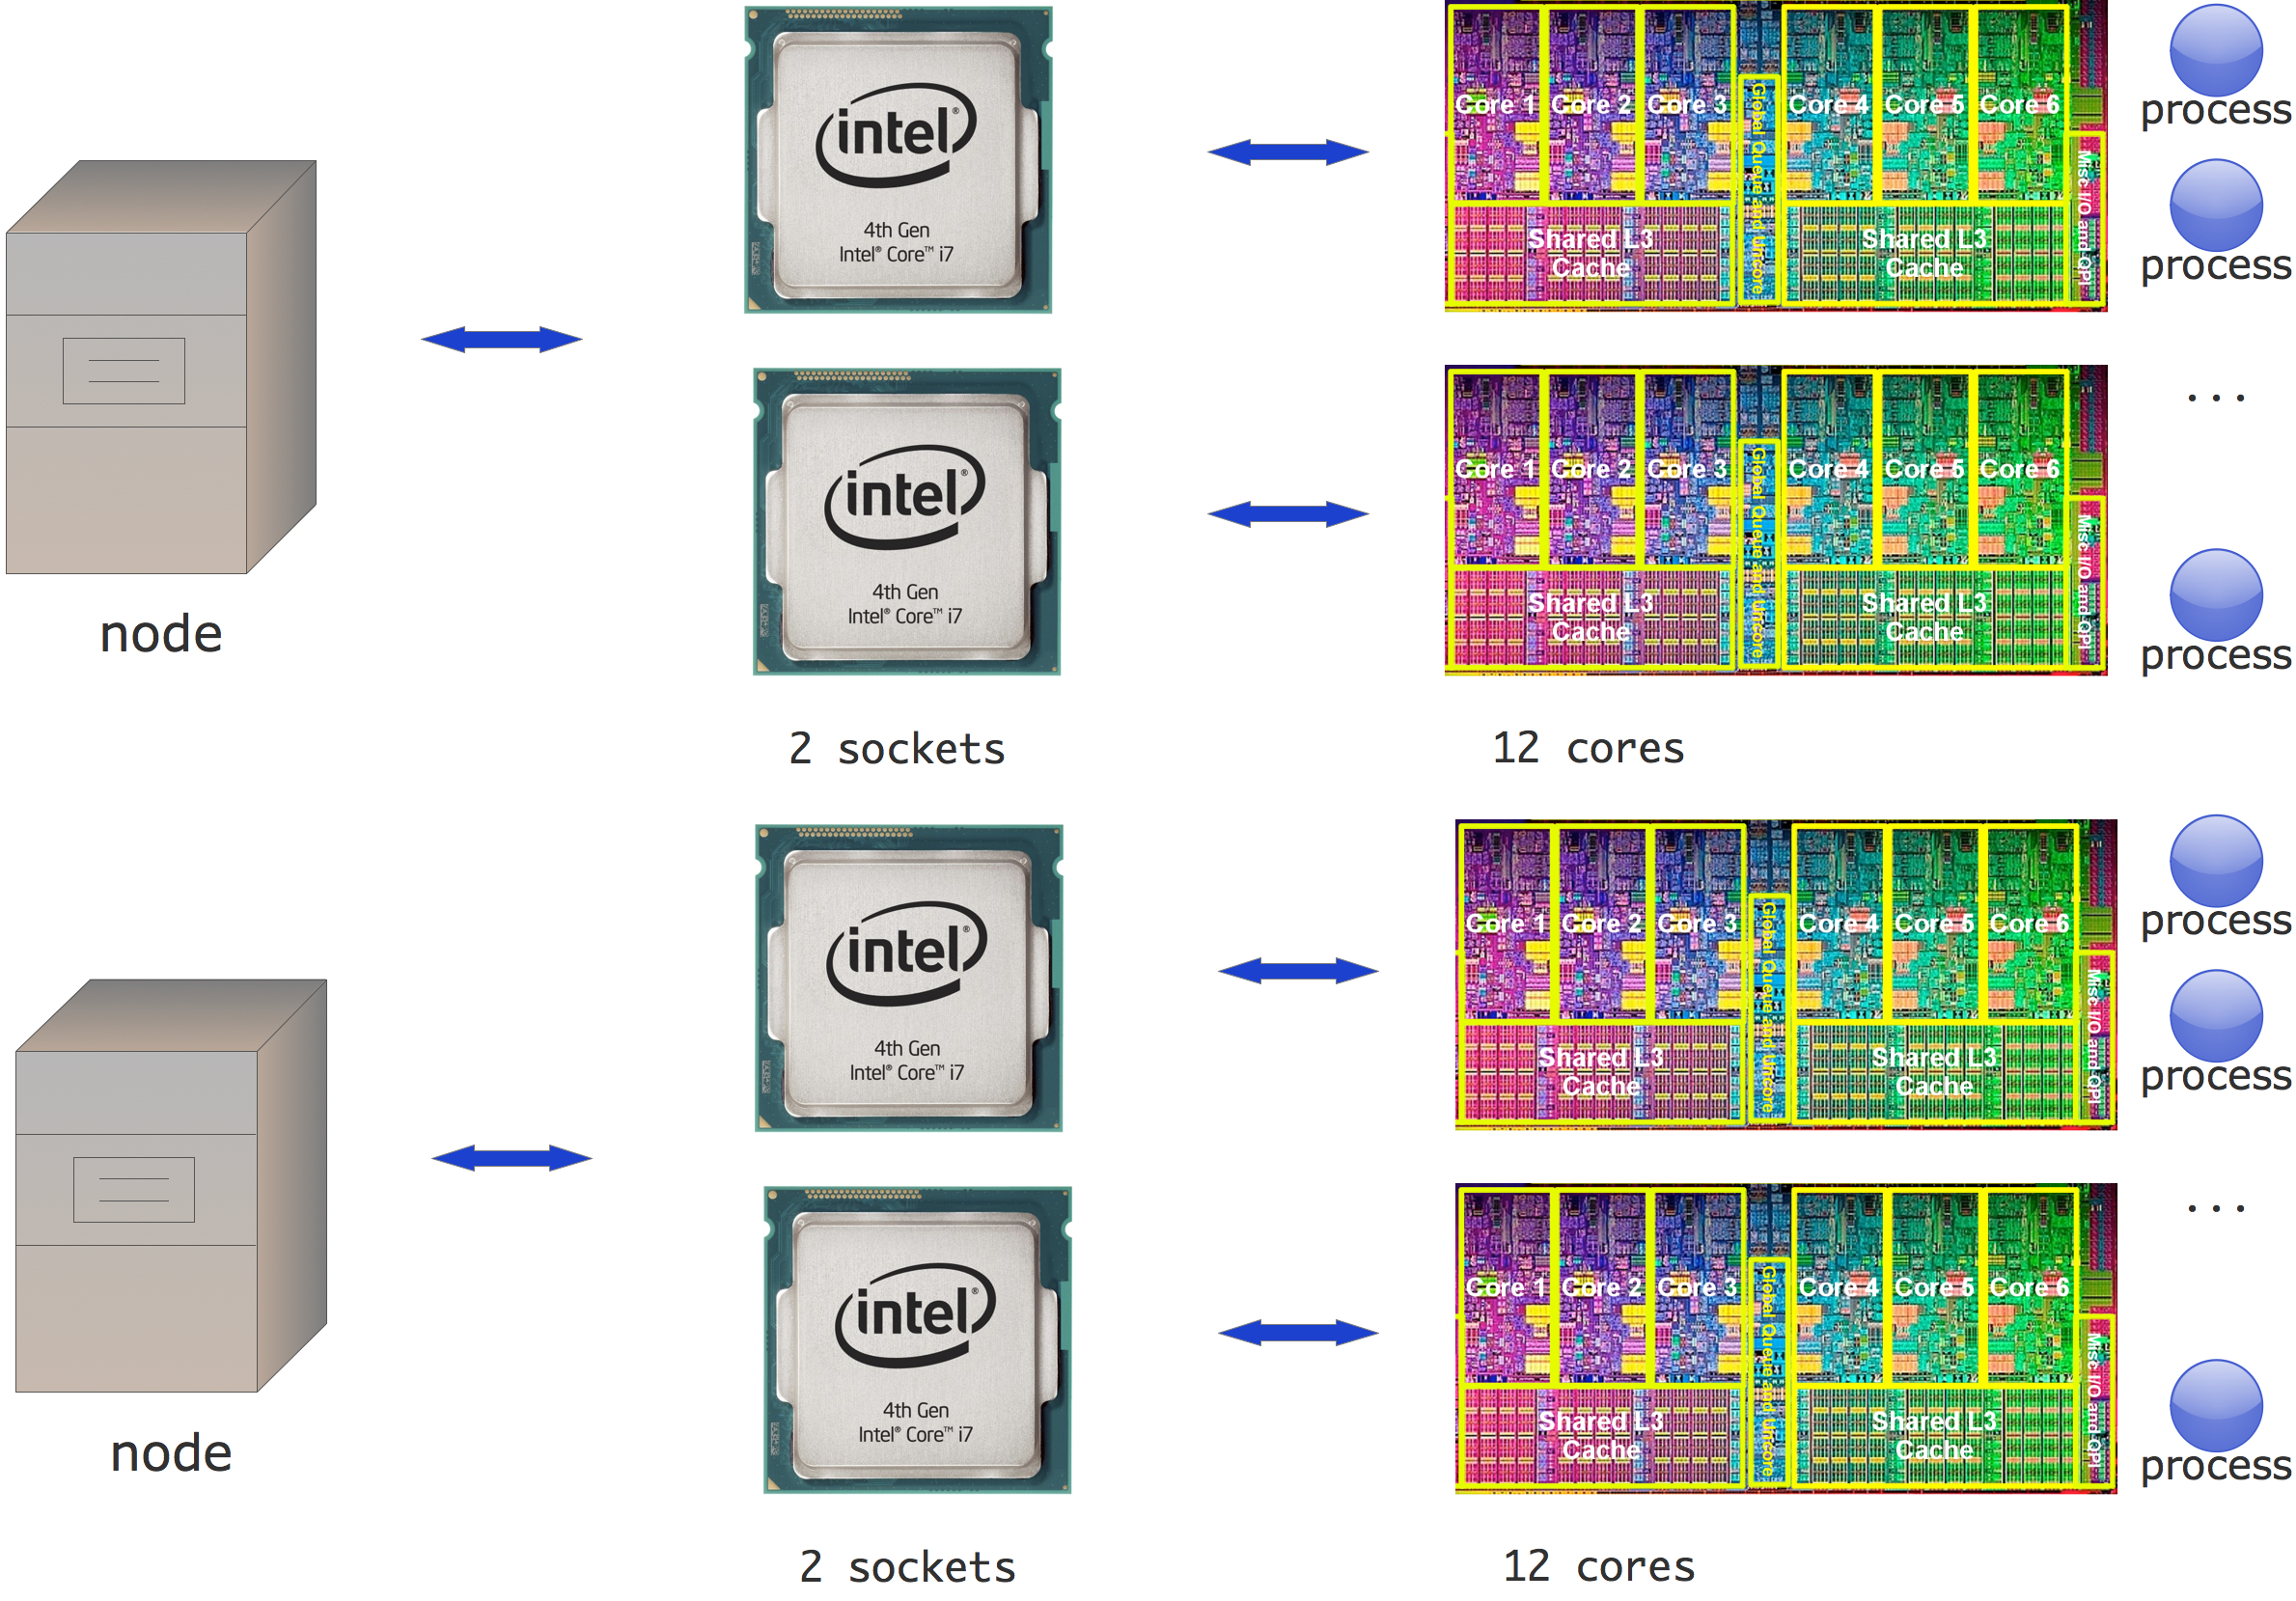
\includegraphics[scale=.11]{mpi-node2}
  \caption{MPI-only cluster structure}
  \label{fig:purempi}
\end{figure}
%

This is somewhat confusing: the old processors needed MPI programming, because
they were physically separated. The cores on a modern processor, on the other hand,
share the same memory, and even some caches. In its basic mode MPI ignores all
of this: each core receives an MPI process and they communicate as if
they are all connected through the same network. In fact, you can't immediately see
whether two cores are on the same node or different nodes.

\Level 1 {Starting and running MPI processes}
\commandref{mpi-init}

The \ac{SPMD} model may be initially confusing. Even though there is
only a single source, compiled into a single executable,
the parallel run comprises a number of independently started MPI
processes (see section~\ref{sec:mpiexec} for the mechanism).

The following exercises are designed to give you an intuition for this
one-source-many-processes setup. In the first exercise you will see
that the mechanism for starting MPI programs starts up independent
copies. There is nothing in the source that says `and now you become parallel'.

The following exercise shows you that 
\begin{exercise}
  \label{ex:hello1}
  Write a `hello world' program, without any MPI in it,
  and run it in parallel with \indextermtt{mpiexec} or your local equivalent. 
\begin{pcse}
    (On TACC machines such as stampede, use \indextermtt{ibrun}.)
\end{pcse}
  Explain the output.
\end{exercise}

To get a useful MPI program you need at least the calls \indexmpishow{MPI_Init}
and \indexmpishow{MPI_Finalize} surrounding your code. See section~\ref{ref:mpi-init}
for their syntax.
\begin{pythonnote}
  There are no initialize and finalize calls: the \n{import} statement
  performs the initialization.
\end{pythonnote}

This may look a bit like declaring `this is the parallel part of a
program', but that's not true: again, the whole code is executed
multiple times in parallel.

\begin{exercise}
  \label{ex:hello2}
  Add the commands \indexmpishow{MPI_Init} and \indexmpishow{MPI_Finalize}
  to your code. Put three different print statements in your code: one before the init,
  one between init and finalize, and one after the finalize. Again explain the output.
\end{exercise}

In the following exercise you will print out the hostname
of each MPI process; see section~\ref{ref:context} for the syntax.
\begin{exercise}
  \label{ex:procname}
  Now use the command \indexmpishow{MPI_Get_processor_name}
  in between the
  init and finalize statement, and print out on what processor your process runs.
  Confirm that you are able to run a program that uses two different nodes.

\begin{tacc}
TACC nodes have a hostname \n{cRRR-CNN}, where RRR is the rack number, C is the chassis
number in the rack, and NN is the node number within the chassis. Communication
is faster inside a rack than between racks!
\end{tacc}
\end{exercise}

\Level 0 {Processor identification}
\commandref{rank-size}

Since all processes in an MPI job are instantiations of the same executable,
you'd think that they all execute the exact same instructions,
which would not be terribly useful.
To distinguish between processors, MPI provides two calls
\begin{enumerate}
\item \indexmpishow{MPI_Comm_size} reports how many processes there are in all; and
\item \indexmpishow{MPI_Comm_rank} states what the number of the process is.
\end{enumerate}
In other words, each process can find out `I~am process~5
out of a total of~20'.

\begin{exercise}
  \label{ex:hello3}
  Write a program where each process prints out message
  reporting its number, and how many processes there are.

  Write a second version of this program, where each process opens a
  unique file and writes to it. \emph{On some clusters this may not be
    advisable if you have large numbers of processors, since it can
    overload the file system.}
\end{exercise}

\begin{exercise}
  \label{ex:hello4}
  Write a program where only the process with number zero
  reports on how many processes there are in total.
\end{exercise}

\Level 0 {Functional parallelism}

Being able to tell processes apart is already enough for some
applications.  Based on its rank, a processor can find its section of
a search space.  For instance, in \indexterm{Monte Carlo codes} a
large number of random samples is generated and some computation
performed on each. (This particular example requires each MPI process
to run an independent random number generator, which is not entirely
trivial.)

\begin{exercise}
  \label{ex:primetest}
  Is the number $N=2,000,000,111$ prime?  Let each process test a
  range of integers, and print out any factor they find.  You don't
  have to test all integers~$<N$: any factor is at most~$\sqrt
  N\approx 45,200$.
\end{exercise}

As another example, in \indexterm{Boolean satisfiability} problems
a number of points in a search space needs to be evaluated. Knowing
a process's rank is enough to let it generate its own portion of the
search space. The computation of the \indexterm{Mandelbrot set} can
also be considered as a case of functional parallelism. However, the
image that is constructed is data that needs to be kept on one
processor, which breaks the symmetry of the decomposition.

Of course, at the end of a functionally parallel run you need to
summarize the results, for instance printing out some total.
The mechanisms for that you will learn next.

%\input chapters/mpi-intro-func

